%==========================================================================
%HTTP/2
%2015/04/08 (rumeda@mikilab.doshisha.ac.jp)
%==========================================================================

\documentclass[a4j,9pt,twocolumn]{jsarticle}
\usepackage{mlm2.0}
\usepackage{epsf}
\pagestyle{plain}


\begin{document}
\twocolumn[
%---------------------------------------------------------------------------
% ヘッダ    書式:\beginheader{回}{年}{月}
%---------------------------------------------------------------------------
\beginheader{161}{2015}{4}


%---------------------------------------------------------------------------
% 発表題目    書式:\title{日本語}{英語} 「\\」で改行できます
%---------------------------------------------------------------------------
\title%
{HTTP/2}%


%---------------------------------------------------------------------------
% 著者名      書式:\author{日本語著者名}{英語著者名}
%---------------------------------------------------------------------------
\author{梅田 玲旺,松井 健人,内村 祐之,市川 燿\\Reo UMEDA,Kento MATSUI,Yushi UCHIMURA,Hikaru ICHIKAWA}

%---------------------------------------------------------------------------


\endheader

%\begin{abstract}
%---------------------------------------------------------------------------
%Recently, a DVD attracts attention along with the image and the digitization of the sound. The standards of these DVD are complicated. So, in this paper, the standards of the DVD are summarized and the DVD of the next generation is refered. 
%---------------------------------------------------------------------------
%\end{abstract}
\vspace{3mm}
]


%よってHTTP/1.1とHTTP/2の違いは以下のTable\ref{table00}である.

%\begin{table}[h]
%\begin{tabular}{|c|l|l|l|}
%\hline
%  & HTTP/1.1 & HTTP/2  \\ \hline
%サーバとの &  複数& 1\\
%接続数&&\\ \hline
%サーバから & ブラウザの & ブラウザの送信順番\\
%返信の順番&送信順番通り&に関係しない \\ \hline
%メッセージの & テキスト形式 & バイナリ形式\\
%表現&&\\ \hline
%ヘッダ圧縮 & なし & あり  \\ \hline
%サーバから & なし & あり  \\
%必要なデータ&&\\
%付与&&\\ \hline


%\end{tabular}
%\caption{HTTP/1.1とHTTP/2の違い}
%\label{table00}
%\end{table}



%\subsection{HTTPヘッダ圧縮}
%HTTPの要求と応答には,「HTTPヘッダ」が含まれている.
%HTTPヘッダはHTTPで通信するためのデータやどんな情報が送られてきたかなどの情報がある.
%\\ しかし,HTTPヘッダの中にはブラウザの情報など同じHTTPヘッダが何度も送られている.
%そのため無駄なデータのやり取りをしていることになる.
%\\ HTTP/2ではHTTPヘッダを圧縮し無駄なデータのやり取りを減少させている.

%---------------------------------------------------------------------------
% 本文
%---------------------------------------------------------------------------

\section{はじめに}
インターネットを多くの人が閲覧しているが
インターネットをするためのソフトであるブラウザを使っている.
ブラウザはサーバにWebページをもらってから画面に表示をしているが
Webページをもらうとき通信をしており,
通信をするためにHTTPが使われている.
\\ HTTPはHypertext Transfer Protocolの略称であり
サーバとブラウザ間でテキストをを主にやり取りするために開発された通信の約束である.
\\ 1990年ごろ物理学者のティム・バーナーズ・リー氏が
組織内という範囲の限られた情報にアクセスするために設計をした.
最初のバージョンであるHTTP/0.9はテキストがメインの簡単なやり取りのみだった.
\\ その後1996年にHTTP/1.0の仕様が公開された.
HTTP/0.9ではテキストを入手するのみだが音楽や画像,動画などの
様々なデータのやり取りに対応し現在のインターネットとほぼ同じようになっている.
\\ 1999年に公開されたHTTP/1.1は複数のデータを効率よく転送するようになっている.
HTTP/1.0では通信路を通信するたびに確保しているが
HTTP/1.1では一度,通信路を繋いだままにする仕様になっている.
しかし,大きい要求があるときは複数要求を送っても
応答が来るまで時間がかかるなど問題があり効率的な
通信ができていない.
\\ 近年はスマートフォンを使いインターネットを観覧する人が非常に多くなっており
1人一台でインターネットがいつでもどこでもできるためインターネット全体の通信量は非常に増えている.
\\ さらに最近のWebサイトではサーバとブラウザ間でやり取りをしなければならないデータの量が増えてきている.そのためページを表示するのに遅くなる要因になる。なので通信を効率よくして通信量を減らす必要がある.



\section{HTTP/2の概要}
HTTP/2ではHTTP/1.1より通信の効率化を目的として,以下の要素から成り立っている.

\begin{itemize}
 \item 通信路の効率化「ストリーム」
 \item バイナリ形式「フレーム」
 \item サーバから追加のデータの応答「サーバプッシュ」
\end{itemize}



\section{HTTP/2の特徴}
\subsection{通信路の効率化「ストリーム」}
HTTP/2では効率のよい通信と速く応答までもらうことを目的とし,
そのためにHTTP/2でのやり取りをするためには相手までの通信路を確保し「ストリーム」という
仮想通信路を作る.
\\ ストリームは通信路の中にさらに小さな通信路があるかのようにしていている.
それぞれにはナンバーが割り振られ「ストリームID」と呼ばれ,
HTTP/2では複数のストリームを使うことで
サーバとのやり取りを同時に複数している.
\\ 同じことをするときHTTP/2では1つの通信路しか使っていないが
HTTP/1.1では複数の通信路を使っている.HTTP/1.1のイメージをFig.\ref{HTTP1.1}に示し,
HTTP/2のイメージをFig.\ref{HTTP200}に示す.


\begin{figure}[h]
\centering
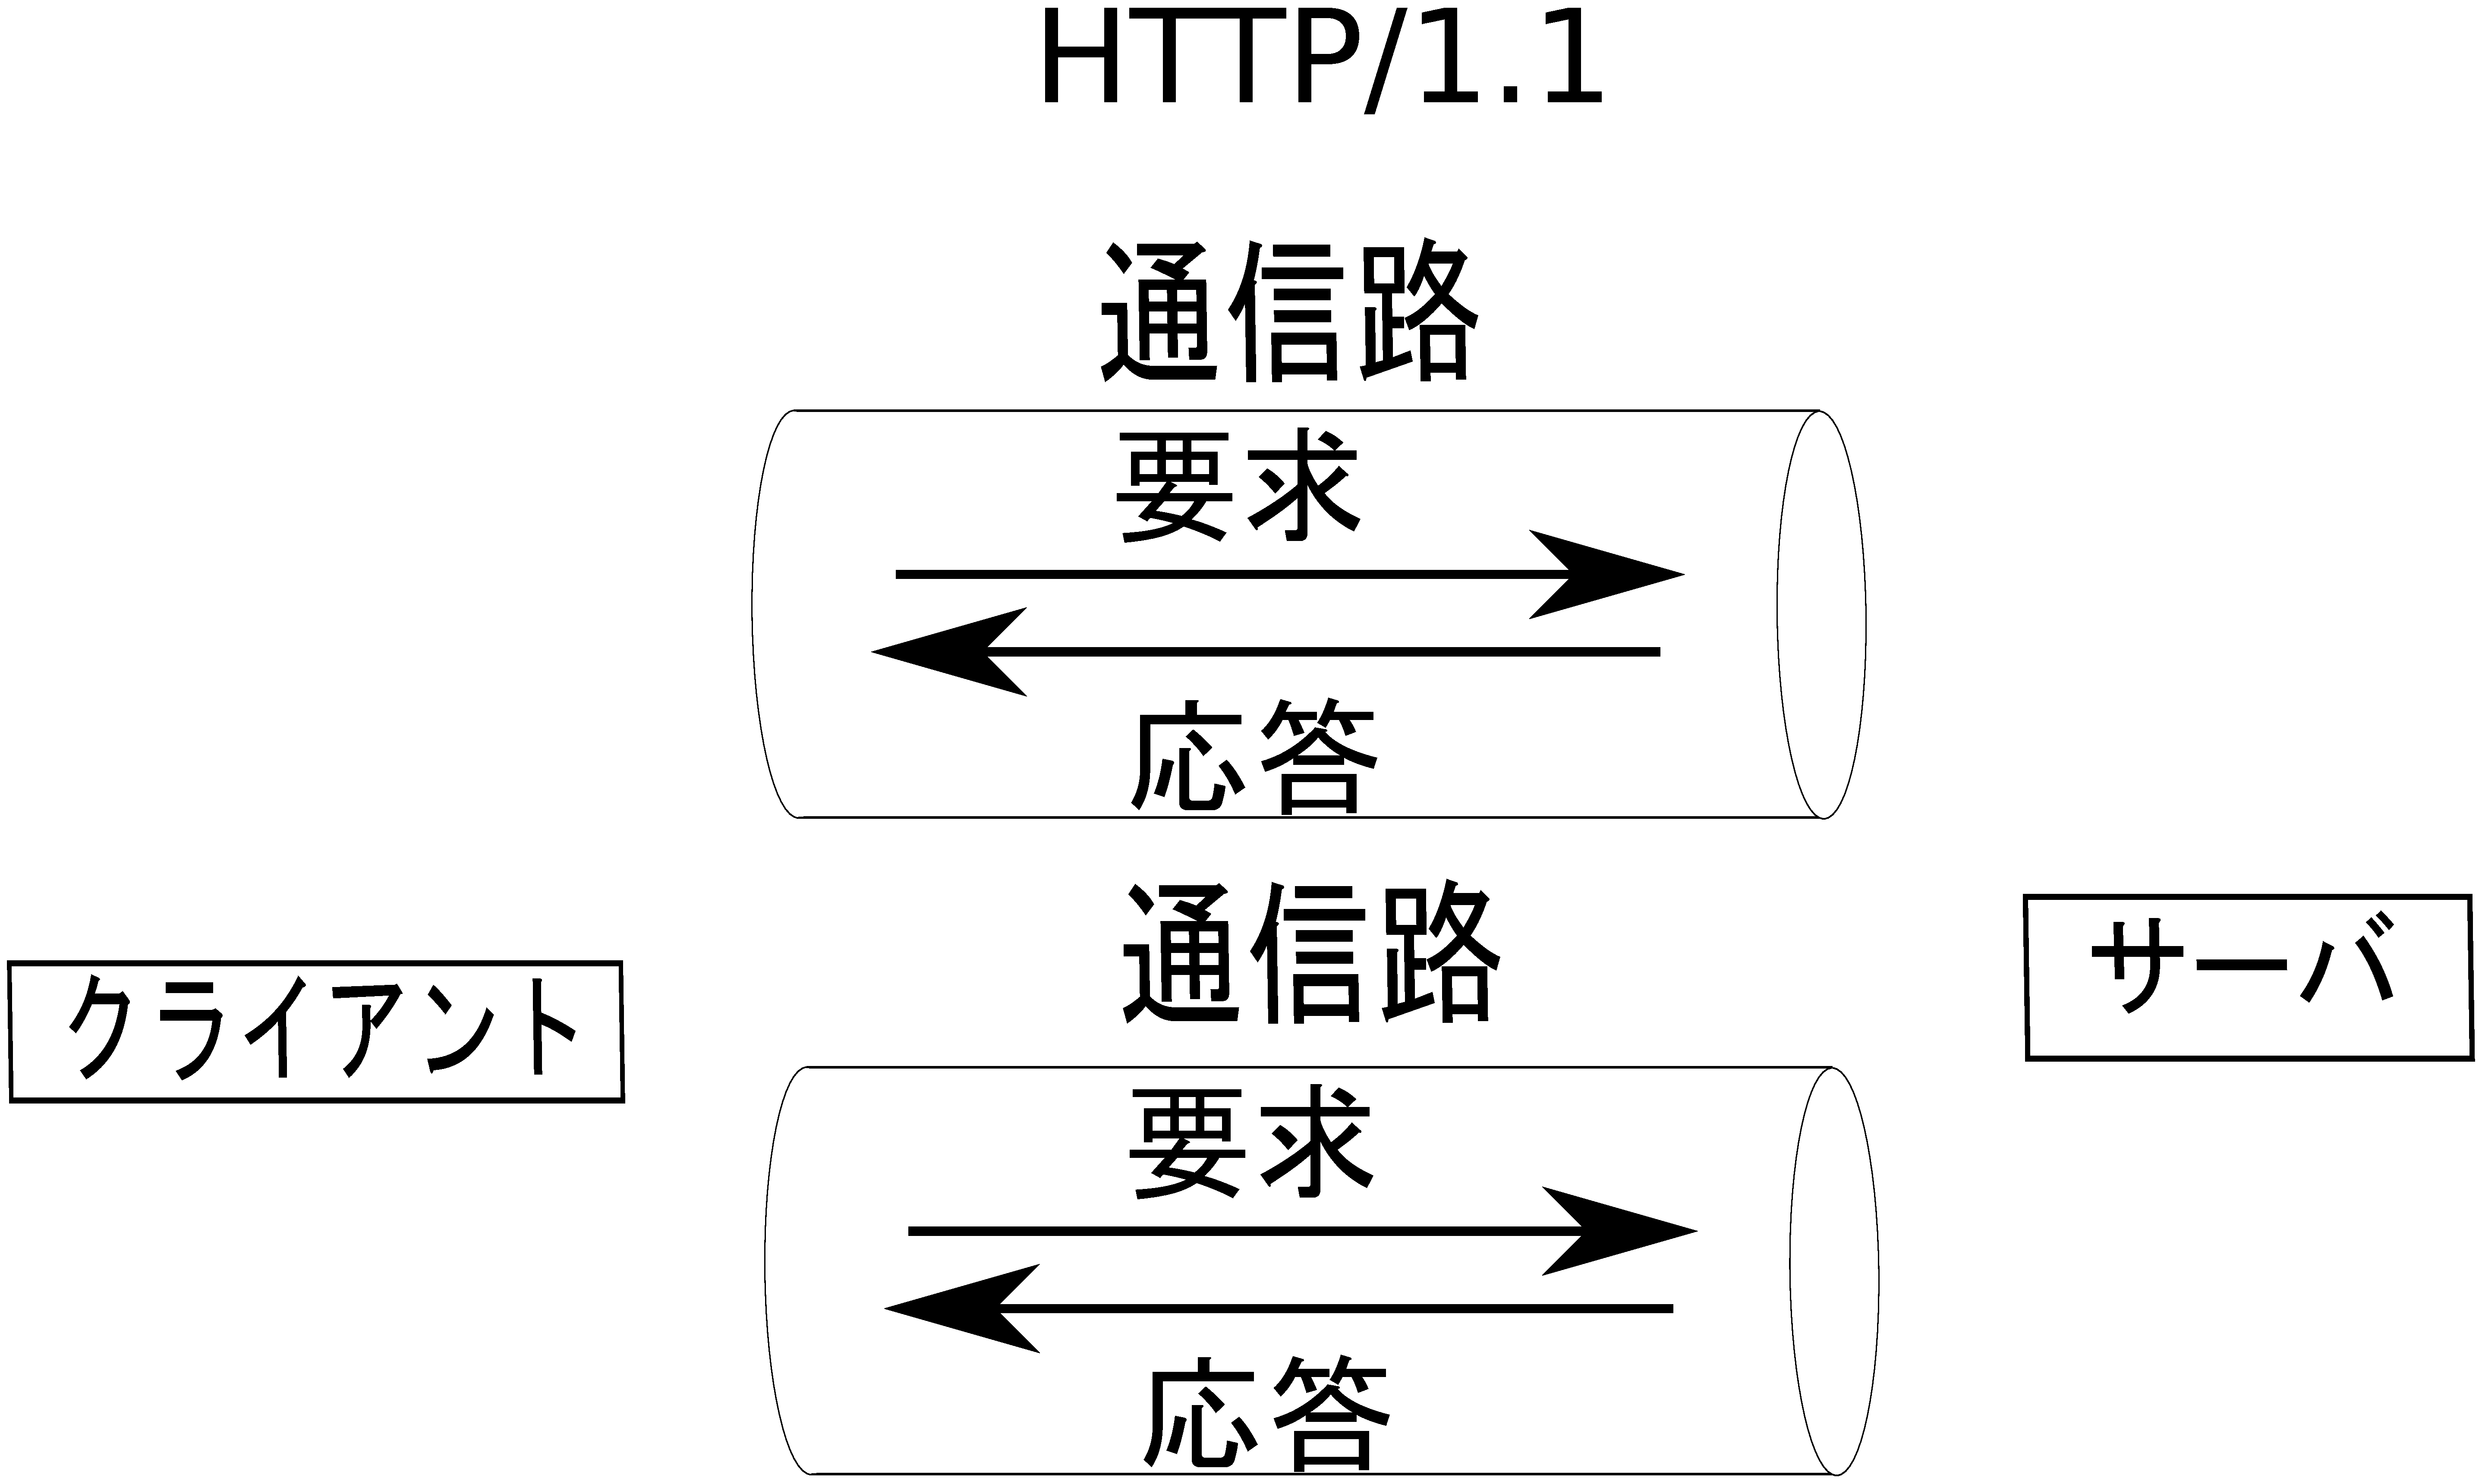
\includegraphics[width=80mm]{img/TCPco5.eps}
\caption{HTTP/1.1の通信路}
\label{HTTP1.1}
\end{figure}




\begin{figure}[h]
\centering
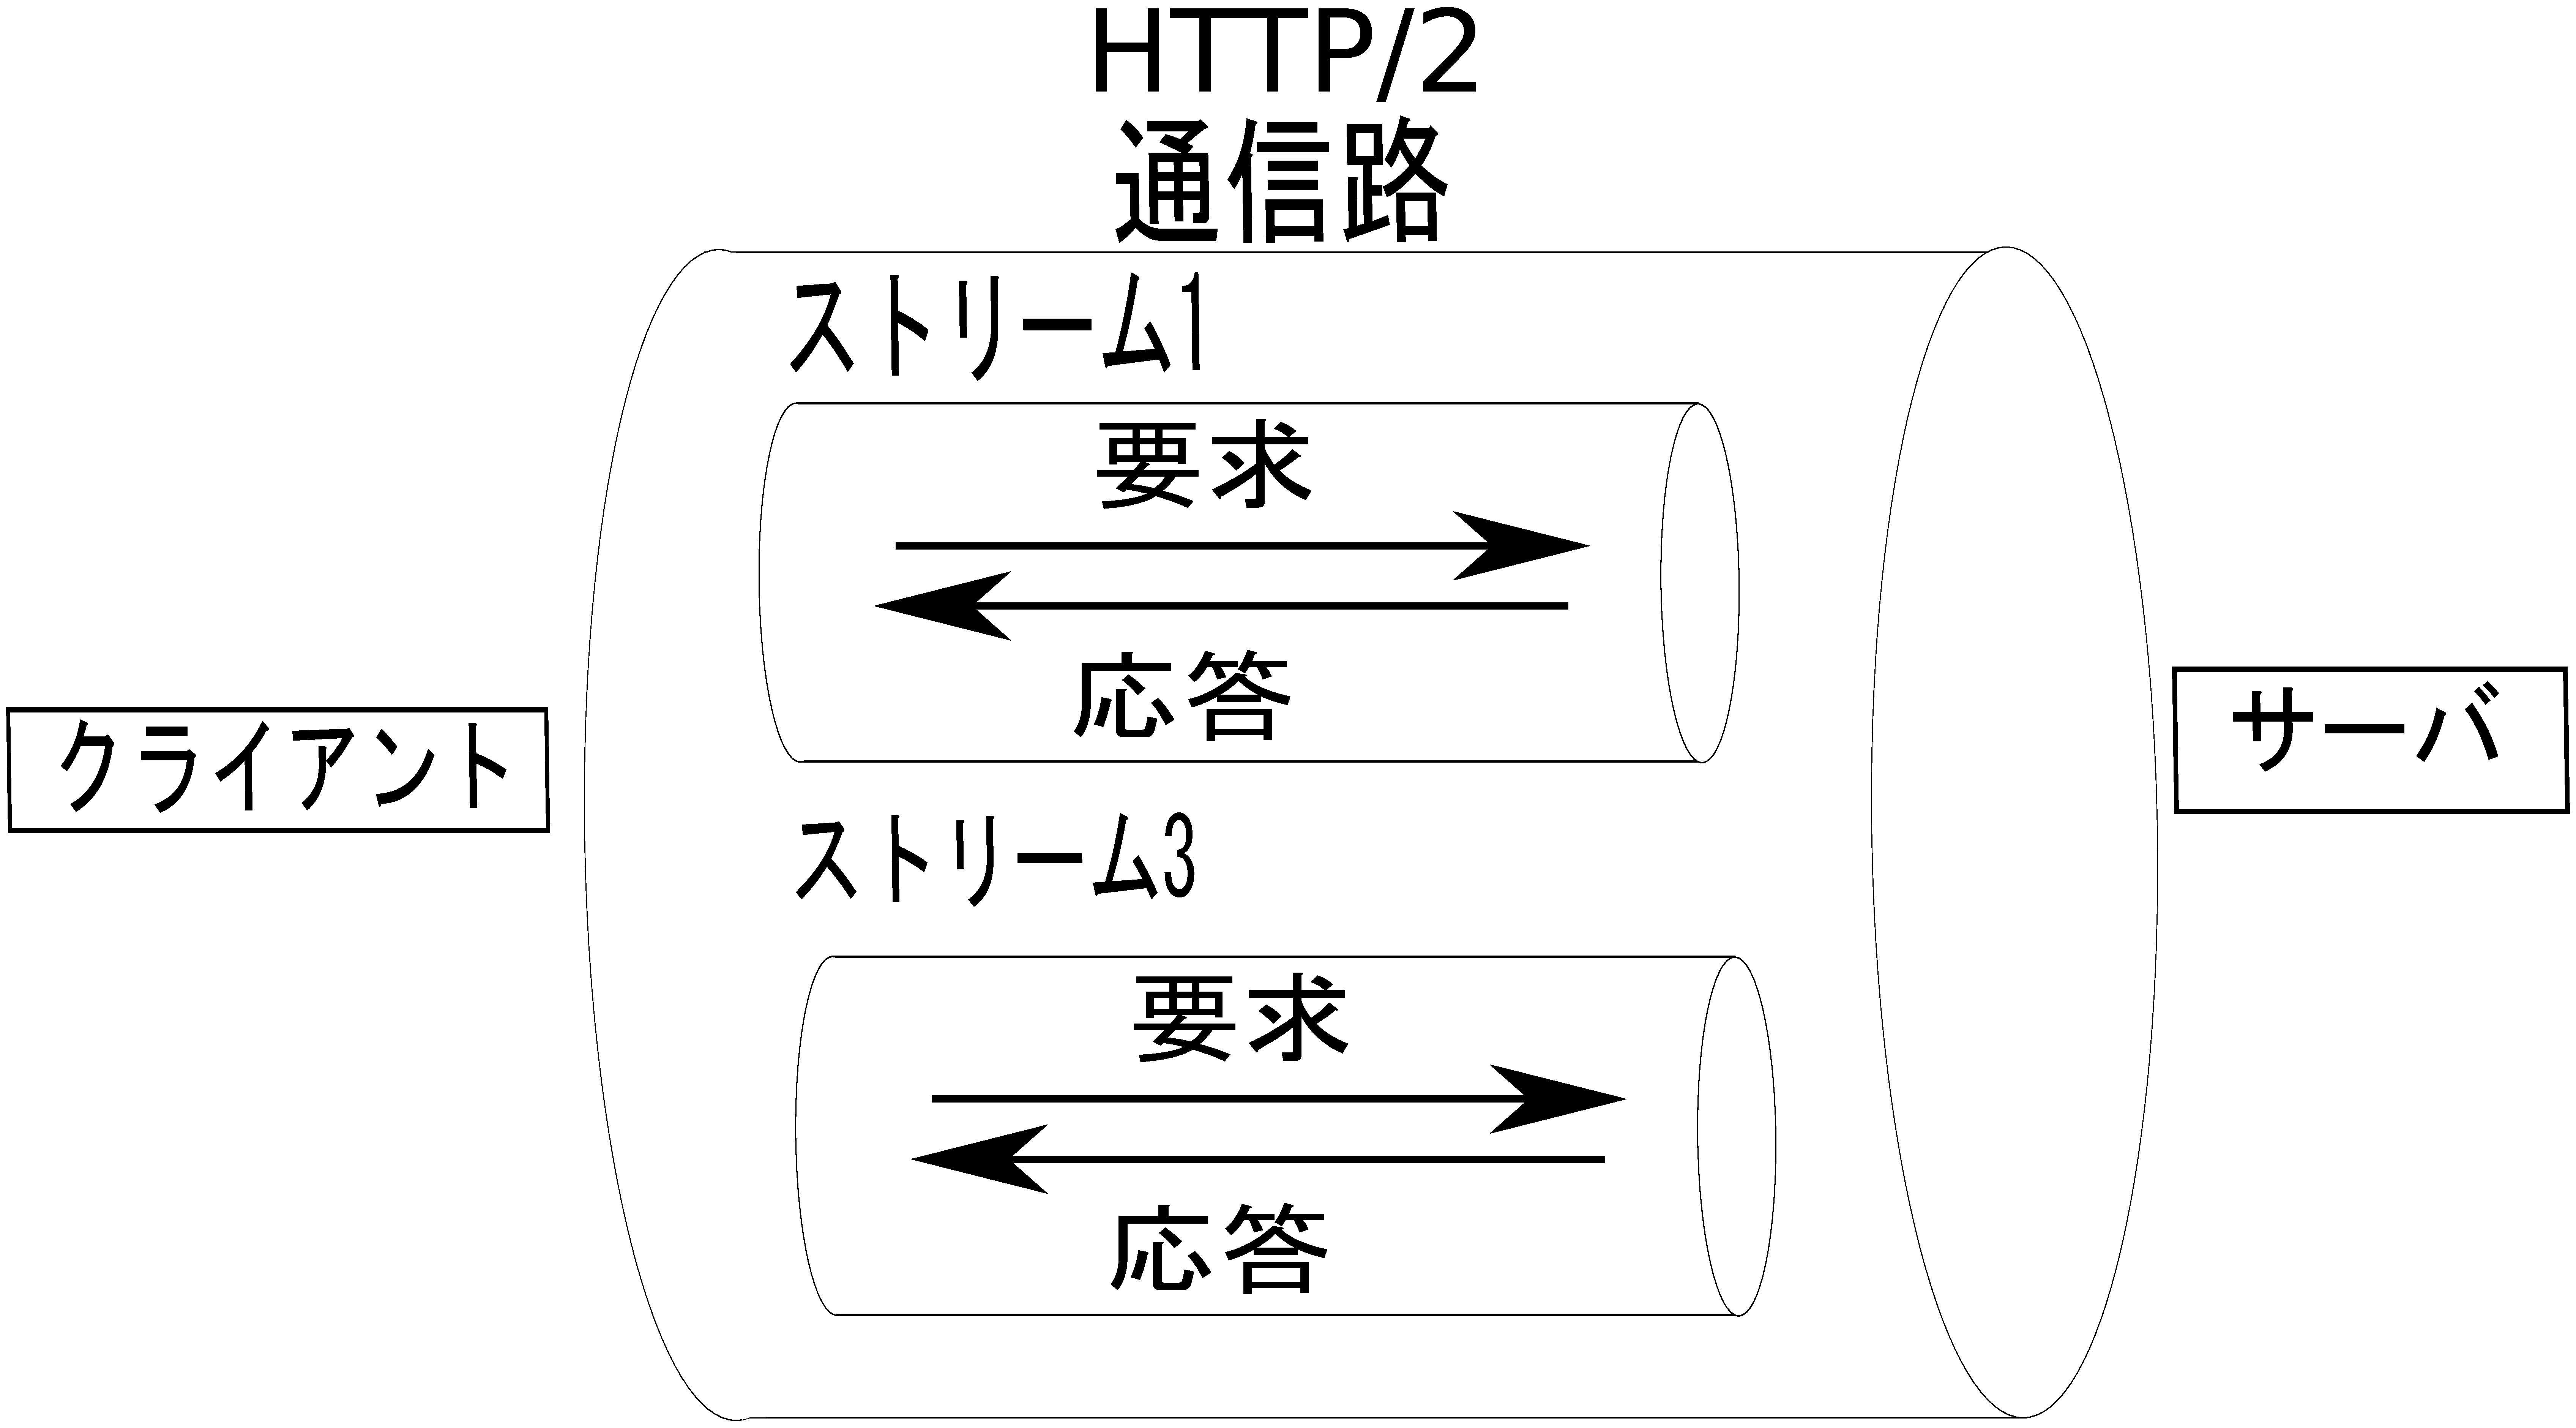
\includegraphics[width=80mm]{img/TCPco6.eps}
\caption{HTTP/2の通信路}
\label{HTTP200}
\end{figure}



このため,HTTP/2はネットワークに対して負担が少なくなる.
ブラウザから複数の要求を送ったとき応答がHTTP/1.1とHTTP/2では異なる.
イメージをFig.\ref{HTTPrespons}に示す.


\begin{figure}[h]
\centering
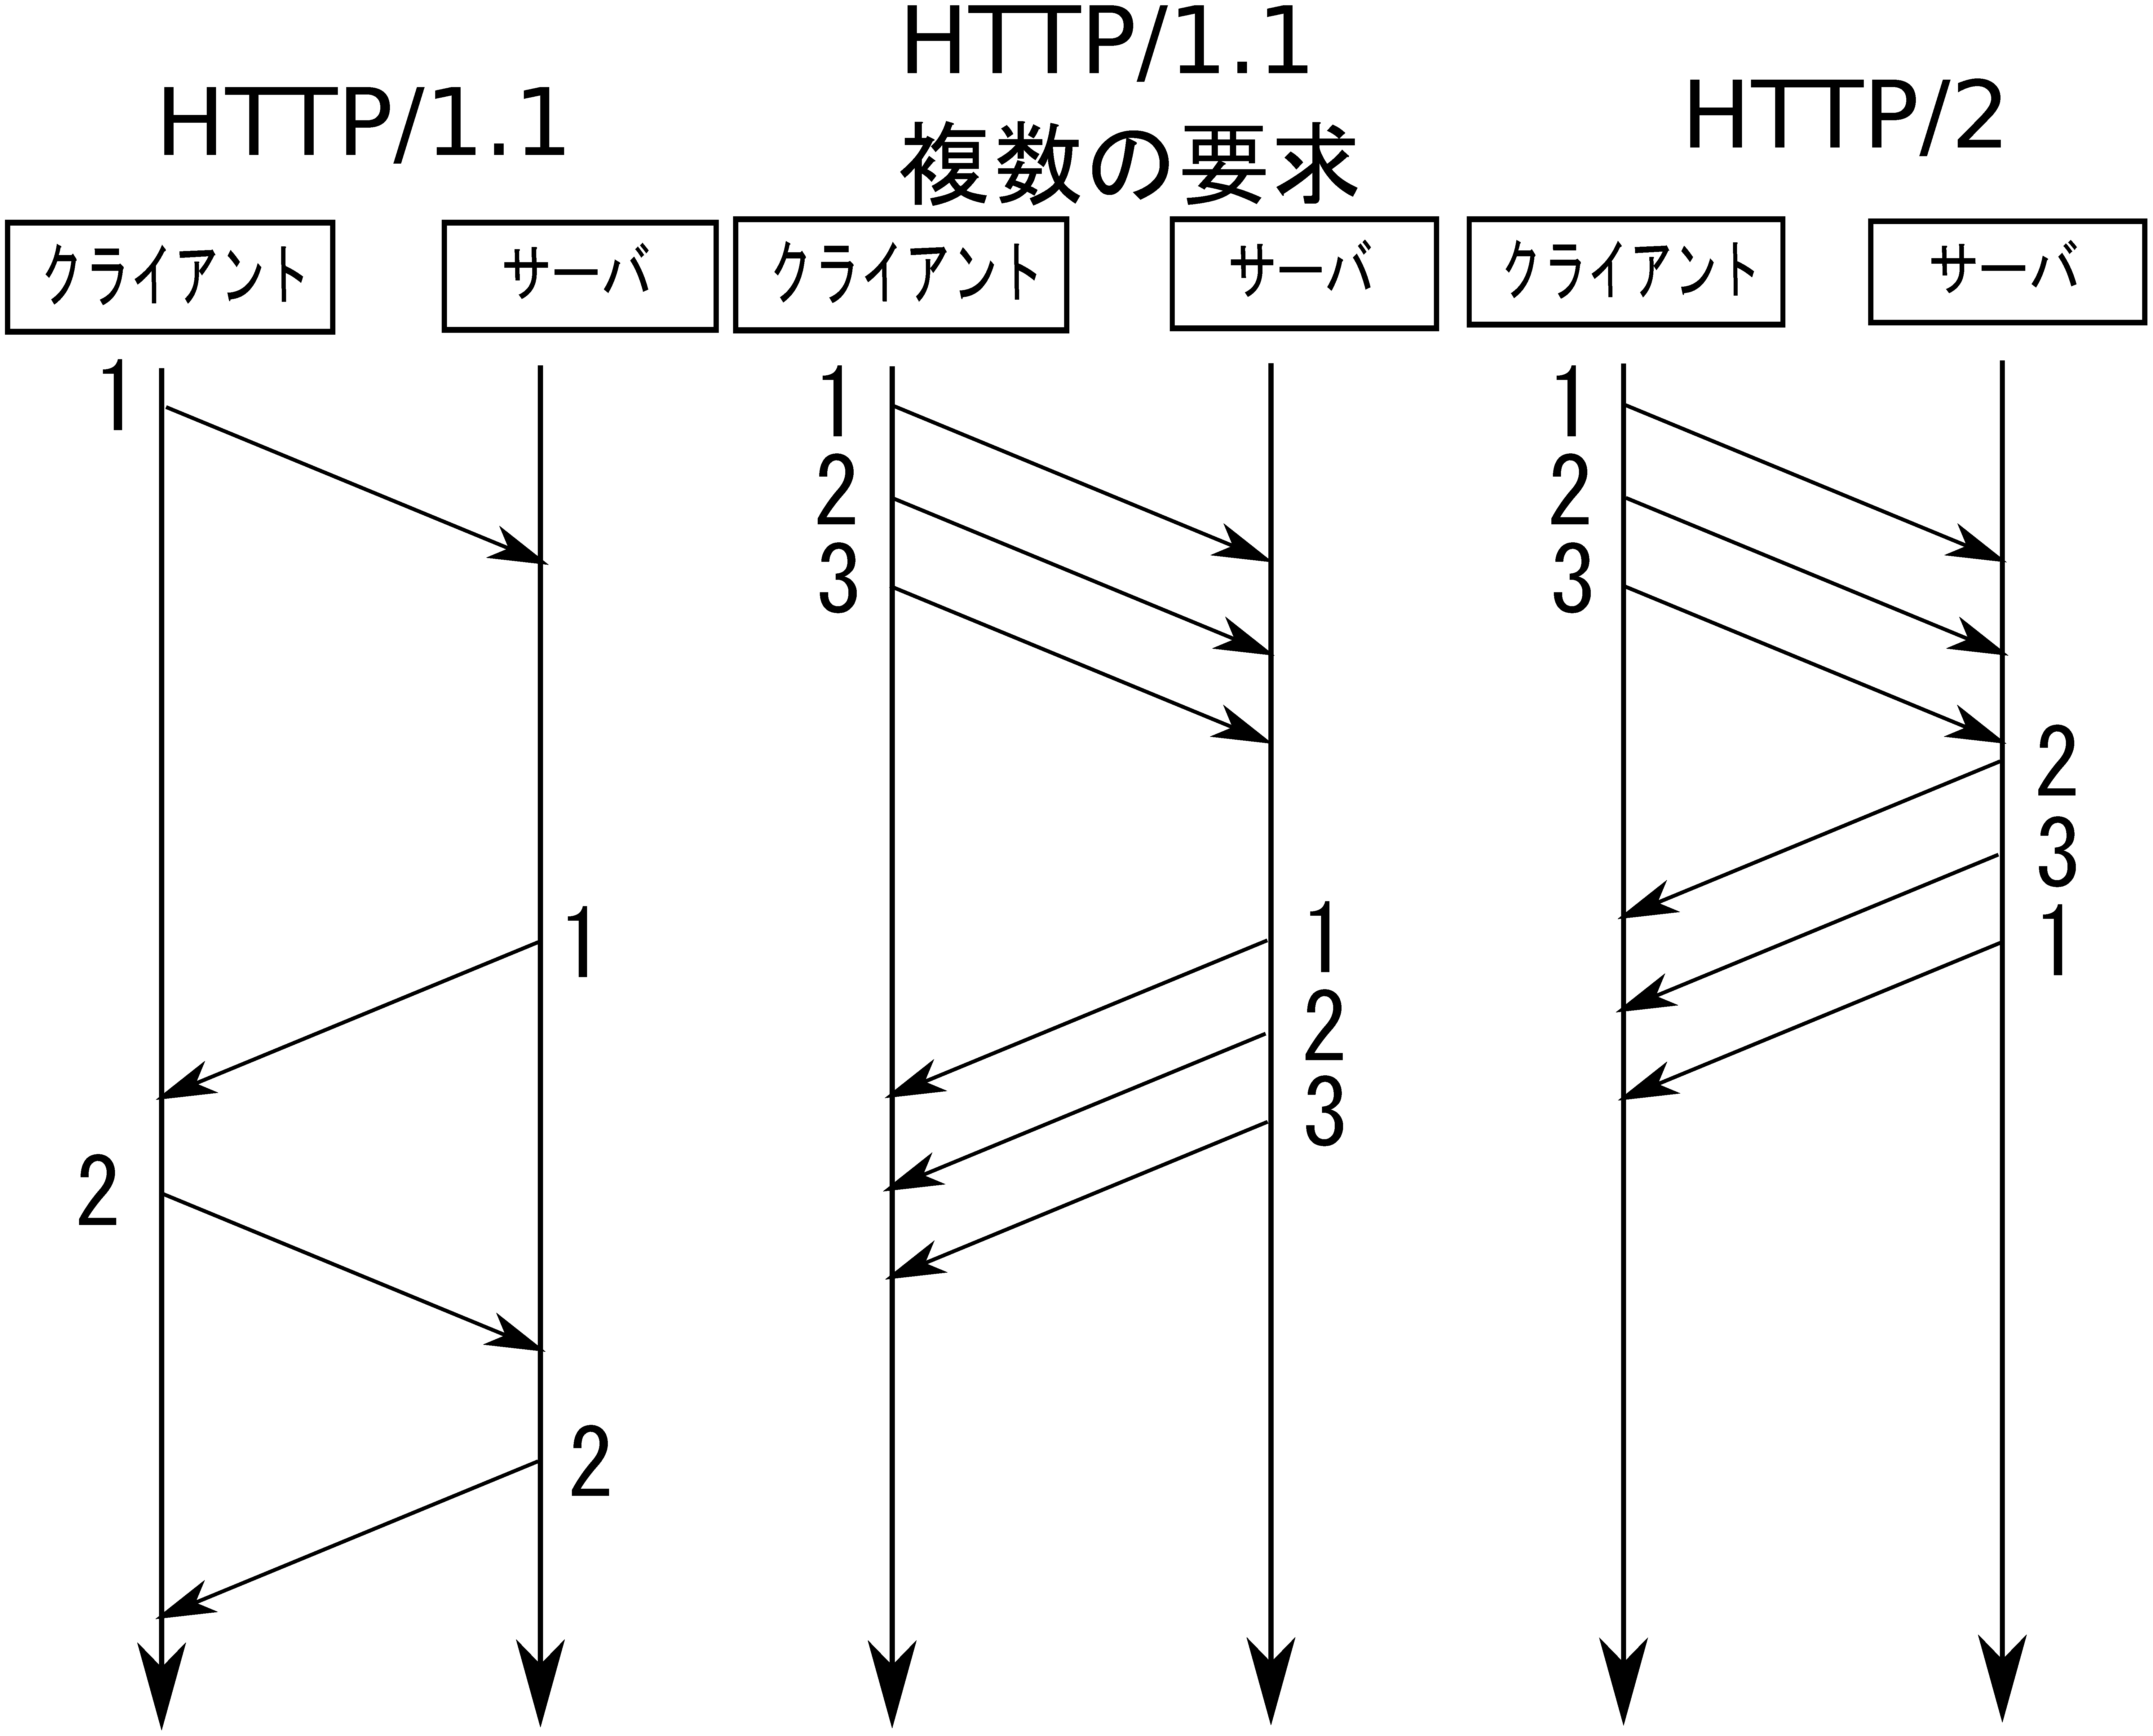
\includegraphics[width=80mm]{img/RR4.eps}
\caption{HTTPの要求と応答}
\label{HTTPrespons}
\end{figure}

HTTP/1.1では要求の順にしか応答は返せない.
しかしHTTP/2では順番に関係なく返すことが出来るため
HTTP/2では処理の速いものから応答を返すことができるようになり
全ての応答が帰ってくる時間が速くなる.
\\ また,HTTP/2ではブラウザ側がストリームに「優先度」をつけることが出来る.
そうすると速く帰ってきて欲しい要求のほうが速く応答が帰ってくるようになる.
\\ 例えば文字の要求を先に送り,後から優先度の高い画像の要求を送ると
画像の応答が速く帰ってくる.



\subsection{バイナリ形式「フレーム」}
HTTP/2になると通信のメッセージ処理を効率的にする目的で「フレーム」という決まった形でやり取りをする.
\\ フレームは以下Fig.\ref{HTTP2frame}のようになる.
\begin{figure}[h]
\centering
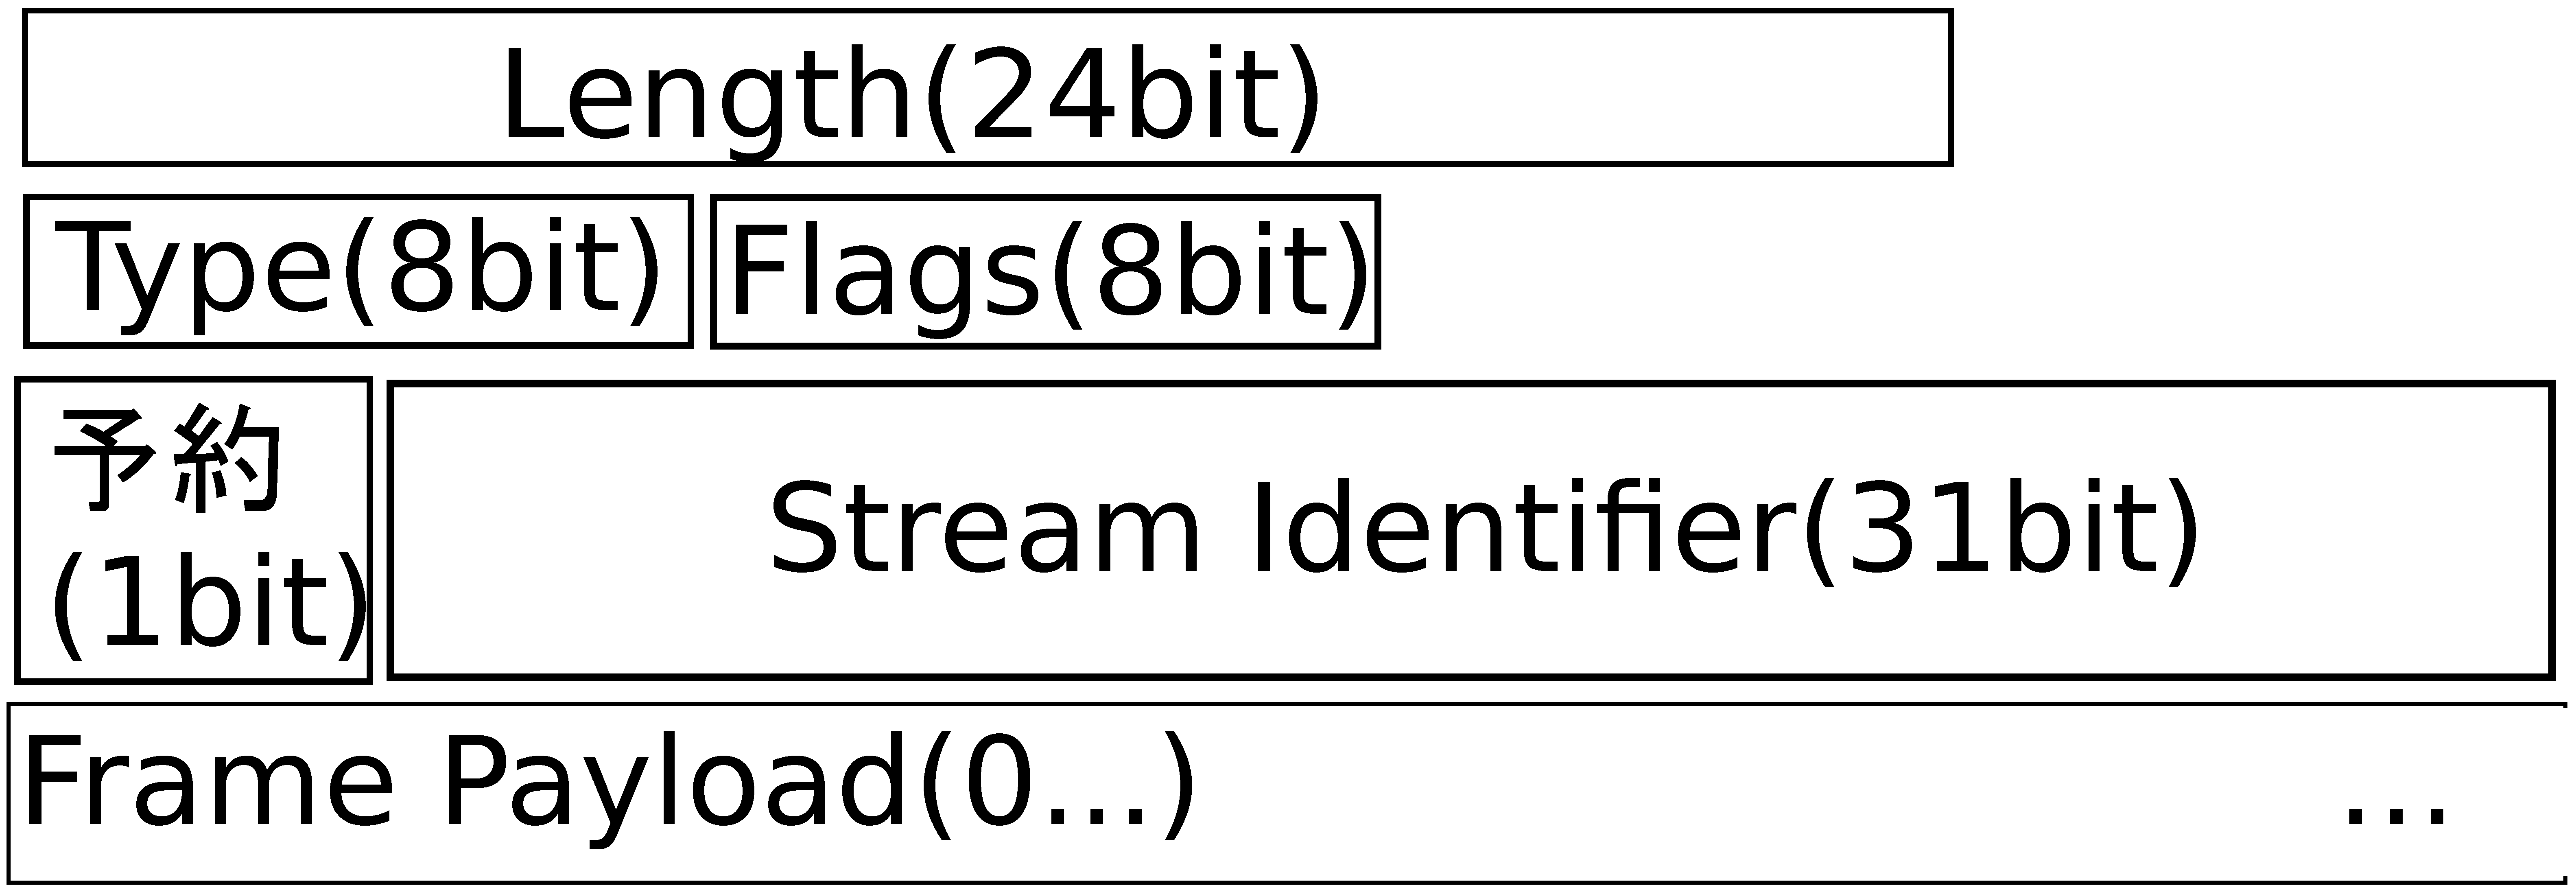
\includegraphics[width=80mm]{img/frame2.eps}
\caption{HTTP/2のフレーム}
\label{HTTP2frame}
\end{figure}

\begin{itemize}
 \item  Length:Frame Payloadの長さ
 \item Type:どんな通信メッセージか
 \item Flags:Typeによっては真偽フラグに使うため予約されている
 \item Stream Identifier:ストリームID
 \item Frame Payload:通信メッセージの内容
\end{itemize}

さらに,HTTP/1.1との差を示すため例としてFig.\ref{AHEAD}を示す.

\begin{figure}[h]
\centering
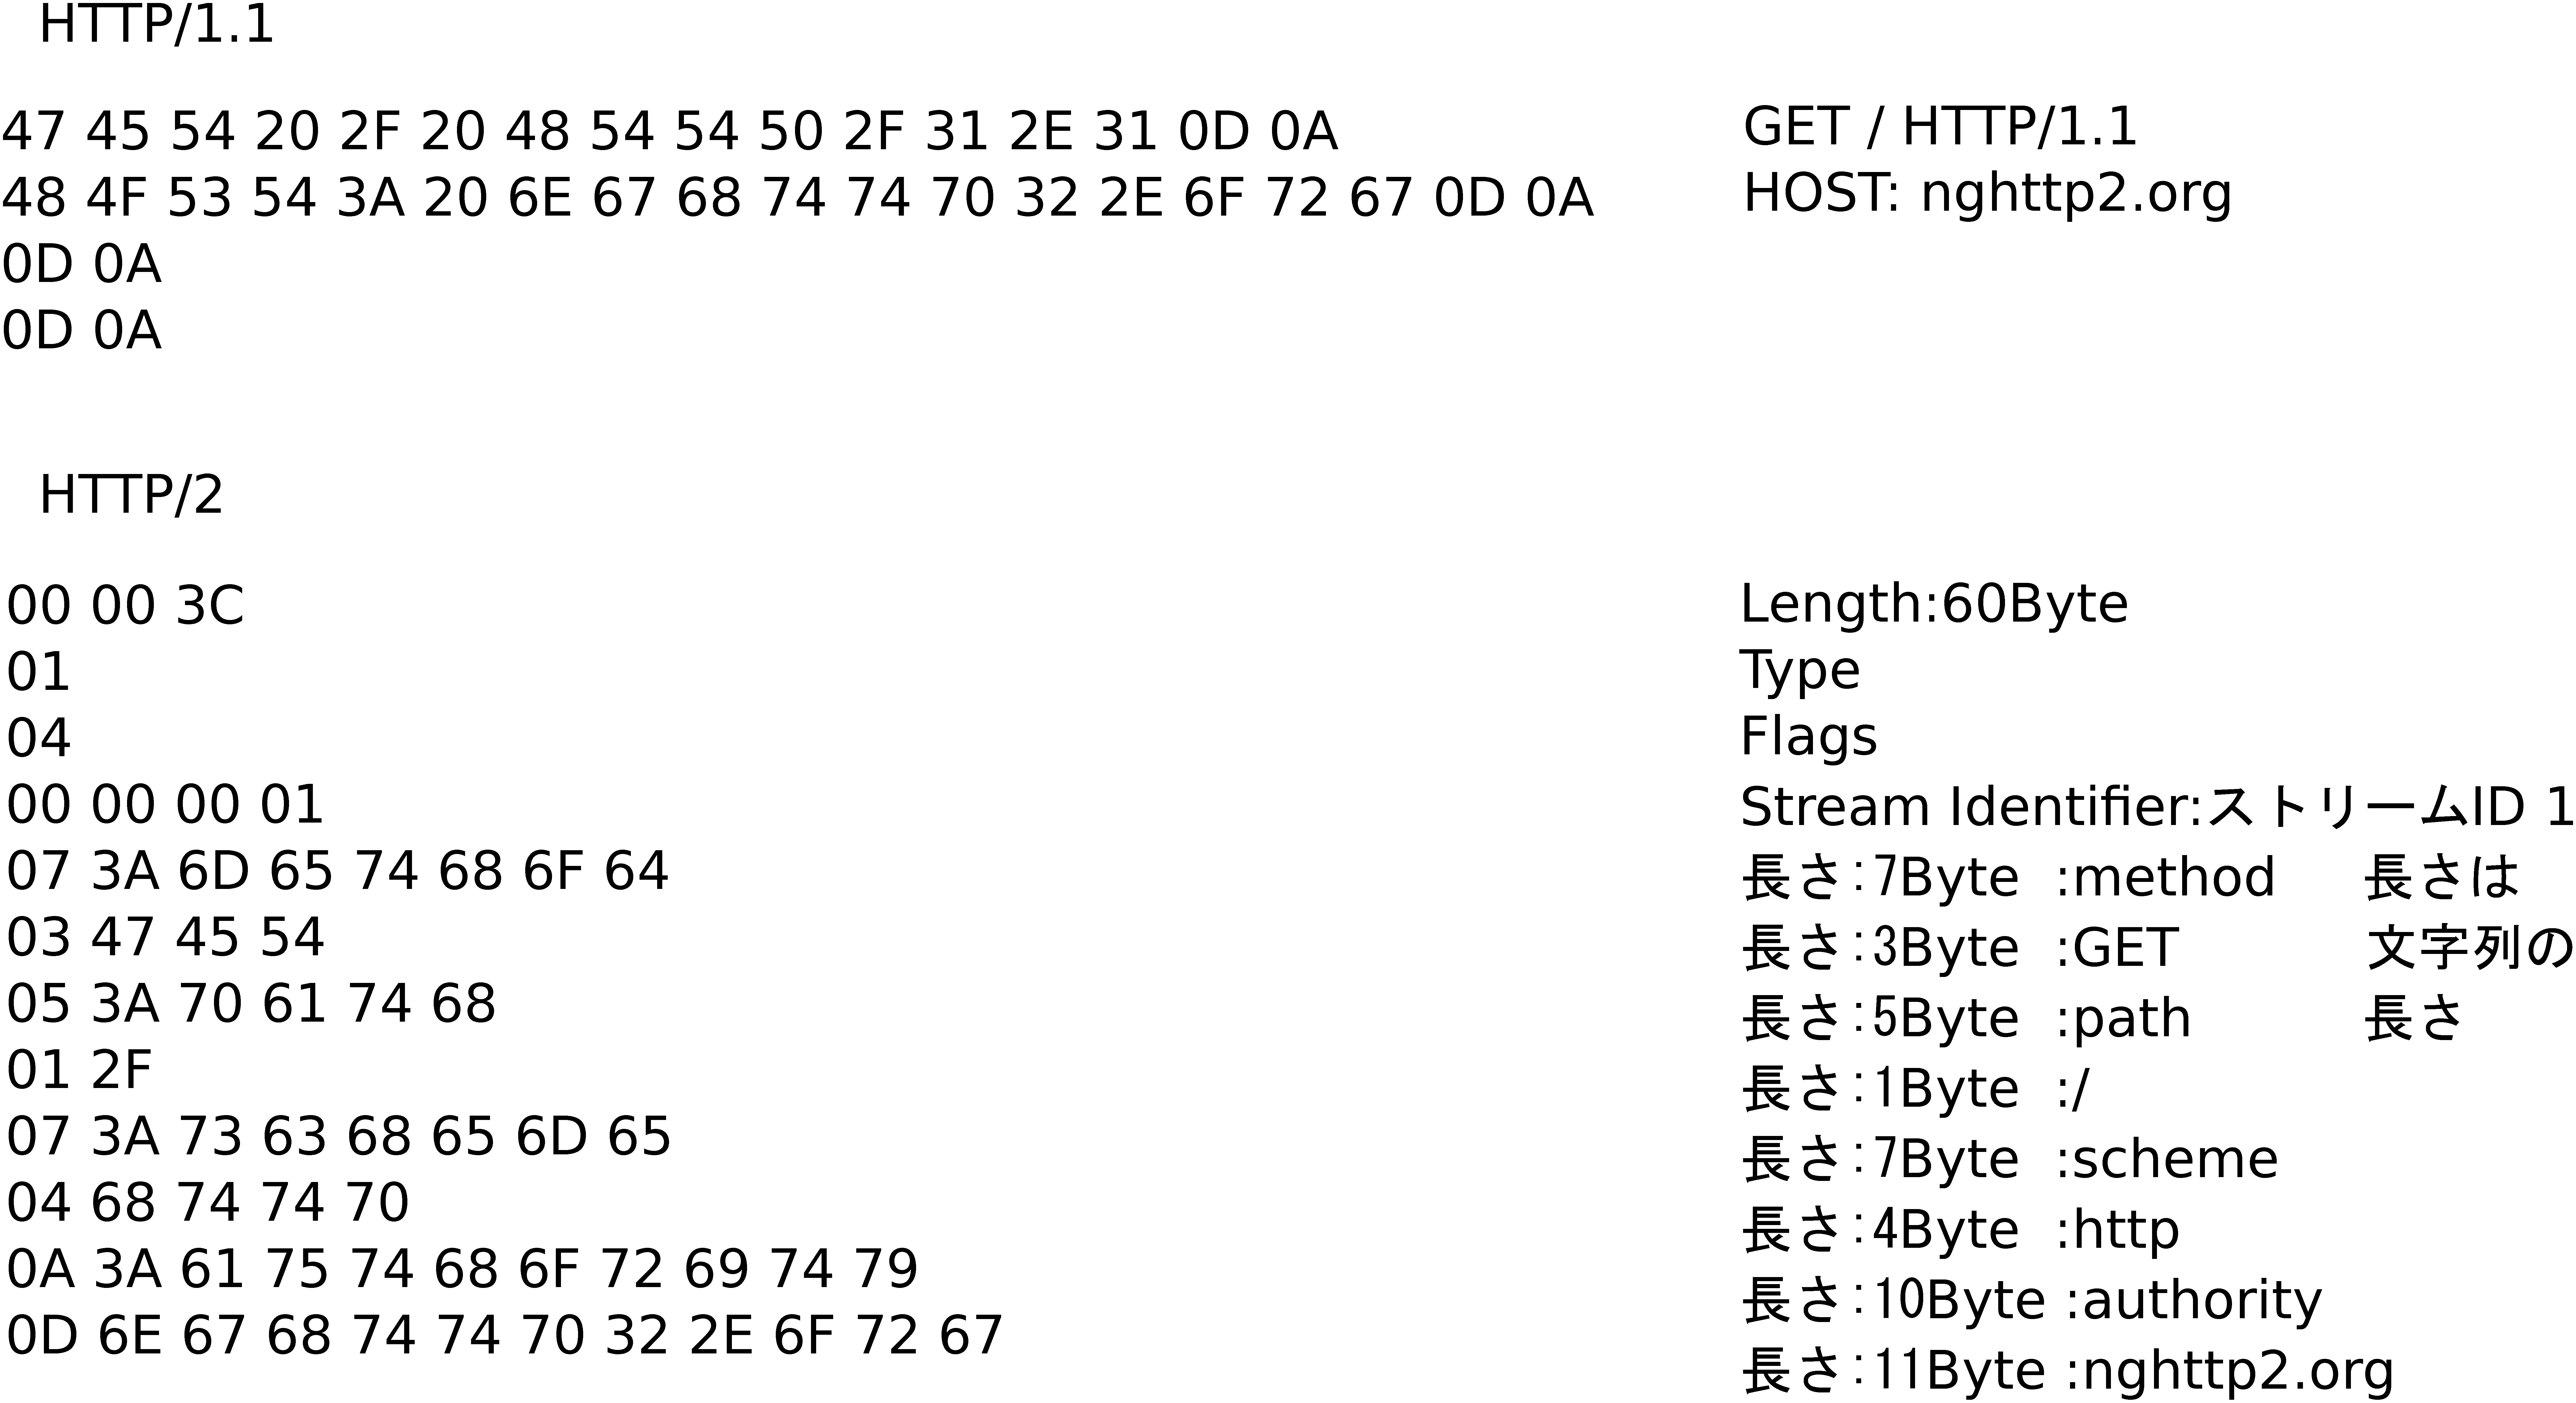
\includegraphics[width=80mm]{img/AHEAD2.eps}
\caption{HTTP/1.1とHTTP/2のメッセージの違い}
\label{AHEAD}
\end{figure}

HTTP/1.1ではメッセージを理解するのに改行や空白などを
確認しなくてはならず処理が大変である.
しかし,HTTP/2は形が決まっておりメッセージの確認が簡単になっている.
\\ 「フレーム」は今までのテキストではなく数値のみであり
バイナリ形式によって決まっており人間には理解しにくい.
しかし,人間には理解しにくくなったがバイナリにしたことで
位置やサイズが決まっているので処理しやすくなり間違いが少なくなる.






\subsection{サーバから追加のデータの応答「サーバプッシュ」}
HTTP/2からはブラウザが要求をサーバに送り,
サーバがブラウザに応答を返すときに要求に関係のあるデータを送ることができる機能
「サーバプッシュ」がある.
これによって速く必要な応答をもらい要求から応答までの時間を減らすことを目的としている.
\\ 例えば,Webページをの要求をブラウザが送ると
HTTP/1.1ではサーバはWebページの情報のみを返している.しかし,HTTP/2からはそのページで表示する画像も一緒に送ることができる.
なのでHTTP/2では後からブラウザが要求を送らなくても
関係しているデータを先にもらうことができる.



\section{HTTP/2今後}
HTTP/2を使うためにはサーバとブラウザの両方が対応して初めて使うことができる.
主要ブラウザの最新バージョンはHTTP/2に対応しており「Windows10」の「Internet Explorer11」,「Firefox36」,「Google Chrome 40」などがある.
\\ Goolge ChromeやFirefoxではセキュリティのある
HTTP/2のみをサポートするなどセキュリティ面での向上も考えられるが
HTTP/2はまだ完全な仕様が決定していないなど
まだまだこれから発展していくものであり恩恵を受けるためにはまだ時間がかかると考えられる.
\\ しかし,Googleやtwitterなどにはすでに導入がされており
これからさらに導入が加速されていくと思われる.




\small
\bibliographystyle{junsrt}
\bibliography{bib}
%------------------------------------------------------------------------------
\end{document}
